\documentclass[letter,12pt]{amsart}

\usepackage{booktabs}   % formal tables
\usepackage{subcaption} % complex figures with subfigures/subcaptions
\usepackage{mathtools,amsthm,amssymb,prftree} % math packages
\usepackage{newtxtext}
\usepackage{newtxmath}
\usepackage{tikz}
\usepackage{tabularx,multirow}
\usepackage{xspace} % smart space
\usepackage{wrapfig}
\usepackage{todonotes}
  \newcommand{\todorosu}[1]{\todo[inline,color=red!10]{(Grigore) #1}}
  \newcommand{\todochen}[1]{\todo[inline,color=blue!10]{(Xiaohong) #1}}
\usepackage{array}
\usepackage{array}
  % see [[https://tex.stackexchange.com/questions/12703/
  % how-to-create-fixed-width-table-columns-
  % with-text-raggedright-centered-raggedlef]]
  \newcolumntype{L}[1]
    {>{\raggedright\let\newline\\\arraybackslash\hspace{0pt}}m{#1}}
  \newcolumntype{C}[1]
    {>{\centering\let\newline\\\arraybackslash\hspace{0pt}}m{#1}}
  \newcolumntype{R}[1]
    {>{\raggedleft\let\newline\\\arraybackslash\hspace{0pt}}m{#1}}
\usepackage{hyperref}

\theoremstyle{default}
  \newtheorem{theorem}{Theorem}[section]
  \newtheorem{proposition}[theorem]{Proposition}
  \newtheorem{conjecture}[theorem]{Conjecture}
\theoremstyle{definition}
  \newtheorem{definition}[theorem]{Definition}
  \newtheorem{remark}[theorem]{Remark}
\theoremstyle{plain}


\newcommand{\prule}[1]{(\textsc{#1})} % (Proof Rule) with small caps

% common maths operators
\newcommand{\cln}{\mathbin{:}}
\newcommand{\ldot}{\mathbin{.}}
\newcommand{\lcma}{\mathbin{,}}
\newcommand{\Colon}{\mathbin{::}}
% common maths symbols
\newcommand{\nats}{\Nbb}
\newcommand{\WF}{\WFcal}
% mathsf fonts
\newcommand{\Setsf}{\mathsf{Set}}
\newcommand{\Propsf}{\mathsf{Prop}}
\newcommand{\Typesf}{\mathsf{Type}}
% mathcal fonts
\newcommand{\Scal}{\mathcal{S}}
\newcommand{\WFcal}{\mathcal{W\!F}}
% mathbb fonts
\newcommand{\Nbb}{\mathbb{N}}

\begin{document}

%% Title information
\title{High-Order Logic in Matching $\mu$-Logic}
\author{Xiaohong Chen}
\author{Grigore Rosu}


\maketitle

\tableofcontents

\section{Simply-Typed $\lambda$-Calculus}

\section{Calculus of Inductive Constructions}

The following is a compact digest of
the comprehensive document of Cic
at the reference website of the Coq theorem prover
at \url{https://coq.inria.fr/distrib/current/refman/language/cic.html}.

\subsection{The formal language of Cic}

\begin{definition}
The set of \emph{sorts},
denoted as $\Scal$, is defined as:
\begin{equation}
\Scal \equiv \{ \Propsf, \Setsf, \Typesf(i) \mid i \in \nats \}
\end{equation}
\end{definition}

\begin{definition}
The set of \emph{terms} is inductively defined as:
\begin{itemize}
\item the sorts $\Setsf, \Propsf, \Typesf(i)$ are terms.
\item variables $x,y,\dots$ are terms.
\item constants $c,d,\dots$ are terms.
\item $\forall x \cln T \lcma U$ is a term, 
where $x$ is a variable and $T,U$ are terms.
If $x$ does not occur in $U$, we write $T \to U$ instead of
$\forall x \cln T , U$.
\item $\lambda x \cln T \ldot u$ is a term,
where $x$ is a variable and $T, u$ are terms.
\item $(t u)$ is a term,
where $t,u$ are terms.
\item $\mathit{let}\ x \coloneq t \cln T \ \mathit{in}\ u$ is a term,
where $x$ is a variable and $t,T,u$ are terms.
\end{itemize}
\end{definition}

\begin{remark}
I didn't find the definition of \emph{types}.
I quote from the reference document that
``from a syntactic point of view, types cannot be distinguished from terms, 
except that they cannot start by an abstraction or a constructor.''
\end{remark}

\subsection{Typing rules in Cic}

\begin{definition}
A \emph{local context}, denoted as $\Gamma$,
is an ordered list of \emph{local declarations},
which can be either a \emph{local assumption} with the form
$x \cln T$ where $T$ is a type,
or a \emph{local definition} with the form
$x \coloneq t \cln T$.
Variables in a local context must be distinct.
If $x$ is declared in $\Gamma$, we write $x \in \Gamma$.
If $x \cln T$ is in $\Gamma$, or there exists a $t$ such that
$x \coloneq t \cln T$ is in $\Gamma$, we write $x \cln T \in \Gamma$.
In the latter case, we also write $x \coloneq t \cln T \in \Gamma$.
The empty local context is denoted as $[]$.
We write $\Gamma \Colon (x \cln T)$ and 
$\Gamma \Colon (x \coloneq t \cln T)$ to mean
the local context $\Gamma$ extended with a local assumption/definition.
We use $\Gamma_1 ; \Gamma_2$ to mean the concatenation of two
local contexts.
\end{definition}

\begin{definition}
A \emph{global environment}, denoted as $E$,
is an ordered list of \emph{global declarations},
which can be either a \emph{global assumption} 
or a \emph{global definition},
but also a \emph{inductive definition}, which we define later.
A global assumption has the form $c \cln T$ for a constant $c$.
A global definition has the form $c \coloneq t \cln T$ for a constant $c$.
The empty global environment is denoted as $[]$.
We write $E ; c \cln T$ and $E ; c \coloneq t \cln T$ to mean
the global environment extended with a global assumption/definition.
\end{definition}

\begin{definition}
The following two forms of judgments are defined simultaneously in 
Figure~\ref{fig:coq_proof_system}:
\begin{itemize}
\item $E[\Gamma] \vdash t \cln T$, which means that the term $t$ is
well-typed and has type $T$ in the global environment $E$
and local context $\Gamma$.
\item $\WF(E)[\Gamma]$, which means that the global environment $E$
is well-formed and $\Gamma$ is valid in $E$.
\end{itemize}
\end{definition}

%\begin{figure}
\renewcommand{\arraystretch}{1}
\begin{tabular}{R{0.3\textwidth}L{0.65\textwidth}}
\prule{W-Empty} &
$\WF([])[]$
\\[0.5cm]
\prule{W-Local-Assume} &
$\prftree
% premise 1
{E[\Gamma] \vdash T \cln s}
% premise 2
{s \in \Scal}
% premise 3
{x \notin \Gamma}
% conclusion
{\WF(E)[\Gamma \Colon (x \cln T)]}
$
\\[0.5cm]
\prule{W-Local-Def} &
$\prftree
% premise 1
{E[\Gamma] \vdash T \cln s}
% premise 2
{s \in \Scal}
% premise 3
{x \notin \Gamma}
% conclusion
{\WF(E)[\Gamma \Colon (x \cln T)]}
$
\end{tabular}
\caption{Coq typing rules}
\label{fig:coq_proof_system}
\renewcommand{\arraystretch}{1}
\end{figure}
\begin{figure}[t]
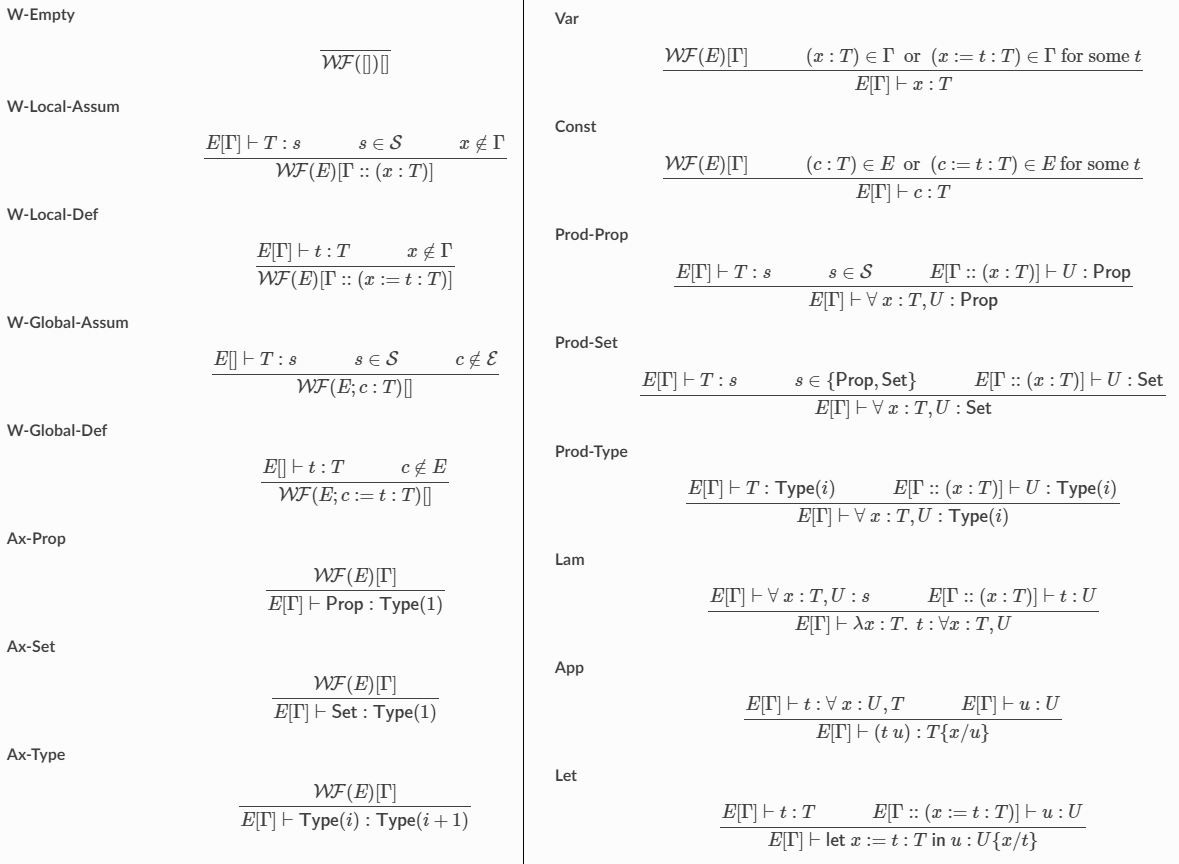
\includegraphics[width=\textwidth]{figs/coq_proof_system.png}
\caption{Cic proof system}
\label{fig:coq_proof_system}
\end{figure}

\end{document}